\documentclass{article}
\usepackage{amsmath}
\usepackage{amssymb}
\usepackage{graphicx}
\title{\textbf{QF605 Project}}
\date{Date: 2019/02/16}
\begin{document}
	\maketitle

\section{Part3 Q1}

\noindent To calculate PV of leg receiving CMS10y semi-annually over the next 5 years, cubic spline interpolation is used between $\alpha$ $\nu$, $\rho$ of $1y$ $\times$ $10y$, $5y\times10y$,$10y\times10y$. SABR parameters for 0.5y expiry follows 1y expiry. Once SABR at different expiries have been interpolated, static replication is used to price each CMS rate and PV is the sum of the discounted values of all CMS rates, multiplied by the day count fraction. Interpolation profiles are given as follow:\\

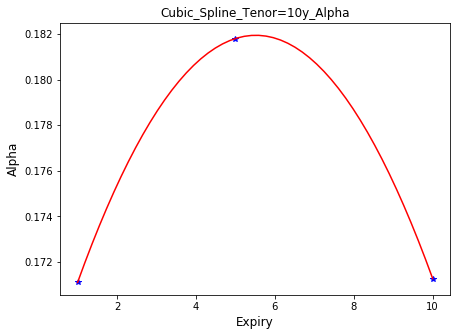
\includegraphics[scale=0.4]{Alpha_10y}\\
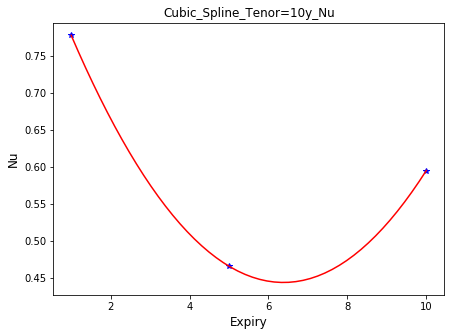
\includegraphics[scale=0.4]{Nu_10y}\\
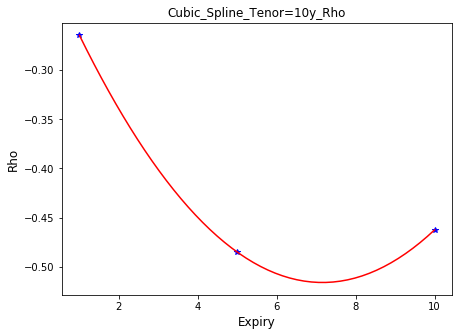
\includegraphics[scale=0.4]{Rho_10y}\\


Similarly, for CMS2y processed quarterly, $\alpha$ $\nu$, $\rho$ can be interpolated between $1y$ $\times$ $2y$, $5y\times2y$,$10y\times2y$, whose profiles are demonstrated below.\\ In addition, quarterly arrangement, more discrete OIS discount rate and Libor Discount rate are interpolated given DF solved in problem.

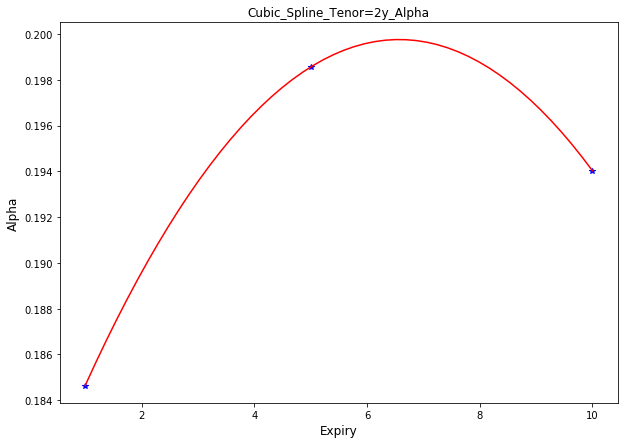
\includegraphics[scale=0.4]{Alpha_2y}\\
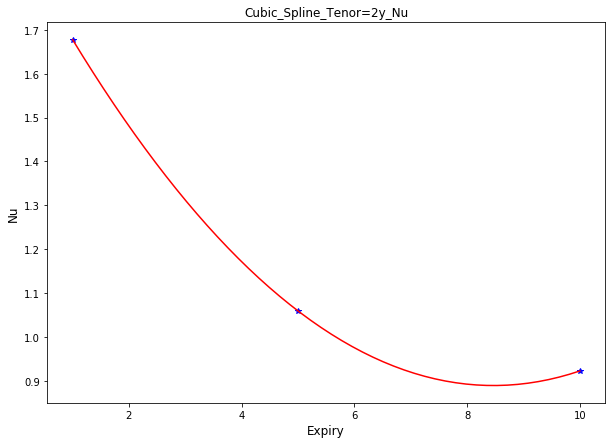
\includegraphics[scale=0.4]{Nu_2y}\\
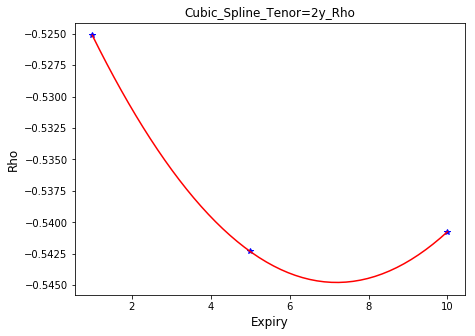
\includegraphics[scale=0.4]{Rho_2y}\\


\end{document}